\documentclass[a4paper]{article}

\usepackage[english]{babel}
\usepackage[utf8]{inputenc}
\usepackage{amsmath}
\usepackage{graphicx}
\usepackage[colorinlistoftodos]{todonotes}

\title{QF603 Group Mini-Project 1}

\author{Group F}

\date{\today}

\begin{document}
\maketitle

\begin{abstract}
Enter a sh ort summary here. What topic do you want to investigate and why? What experiment did you perform? What were your main results and conclusion?
\end{abstract} 

\section{Task 1}
\label{sec:introduction}

\subsection{Verification of DJIA index}
The summation of the 30 component stock prices : 3742.98 \linebreak 
DJIA index value :
$$ DJIA index = \frac{3742.98}{0.14748071991788} = 25379.453002969884
$$

\subsection{Findings about S\&P 500}
The popular S\&P 500, known in full as the Standard \& Poor’s 500, once took humbler forms. First called “The Composite Index”, the initial form of the S\&P 500 tracked only a handful of stocks when Poor’s Publishing introduced it in 1923. The index saw its number of tracked stocks increase to 90 in 1926, and in 1941, Poor’s Publishing merged with Standard Statistics to form Standard \& Poor’s Corporation. It was only until 4 March 1957 that the index saw its number of tracked stocks increase to 500 and its name changed to the “S\&P 500” that we are all more familiar with in recent years. Only a handful of the S\&P 500’s original members, such as Coca-Cola, Pfizer and PepsiCo are still in the index today.

Unlike the older Dow Jones Industrial Average (also known as “the Dow”), which assigns index component weights by price, the S\&P 500 weighs its components by market capitalisation. It is for this reason, amongst many others, that the S\&P 500 is sometimes regarded as more representative of the U.S. equity market. The S\&P 500’s superior breadth (the S\&P 500 tracks 505 stocks, the Dow’s tracks 30) and depth (the S\&P 500 reflects stocks making up \% of the U.S. equity market, compared to the Dow’s \%) of coverage compared to the Dow’s are often also other pull factors for institutional investors. It is also noteworthy that all of the Dow’s 30 components are also included in the S\&P 500, so investors seeking a broader version of Dow may consider the S\&P 500 as one of their viable options.

The S\&P 500’s price is computed by simply dividing the sum of the weighted prices of its components by a divisor, which is adjusted in the event of stock splits, spinoffs or any other event which may unduly and numerically alter the component stock’s price. Components of the S\&P 500 have to undergo a selection process by a committee before being included in the index.  When being considered for inclusion into the S\&P 500, a stock is assessed on nine different criteria, with domicile, exchange listing, organisational structure \& share type, market capitalisation and liquidity just being just a few of said criteria. Usually, only large cap and heavily traded stocks make it into the S\&P 500.

\subsection{Time series of the two indexes}

\begin{figure}[h]
	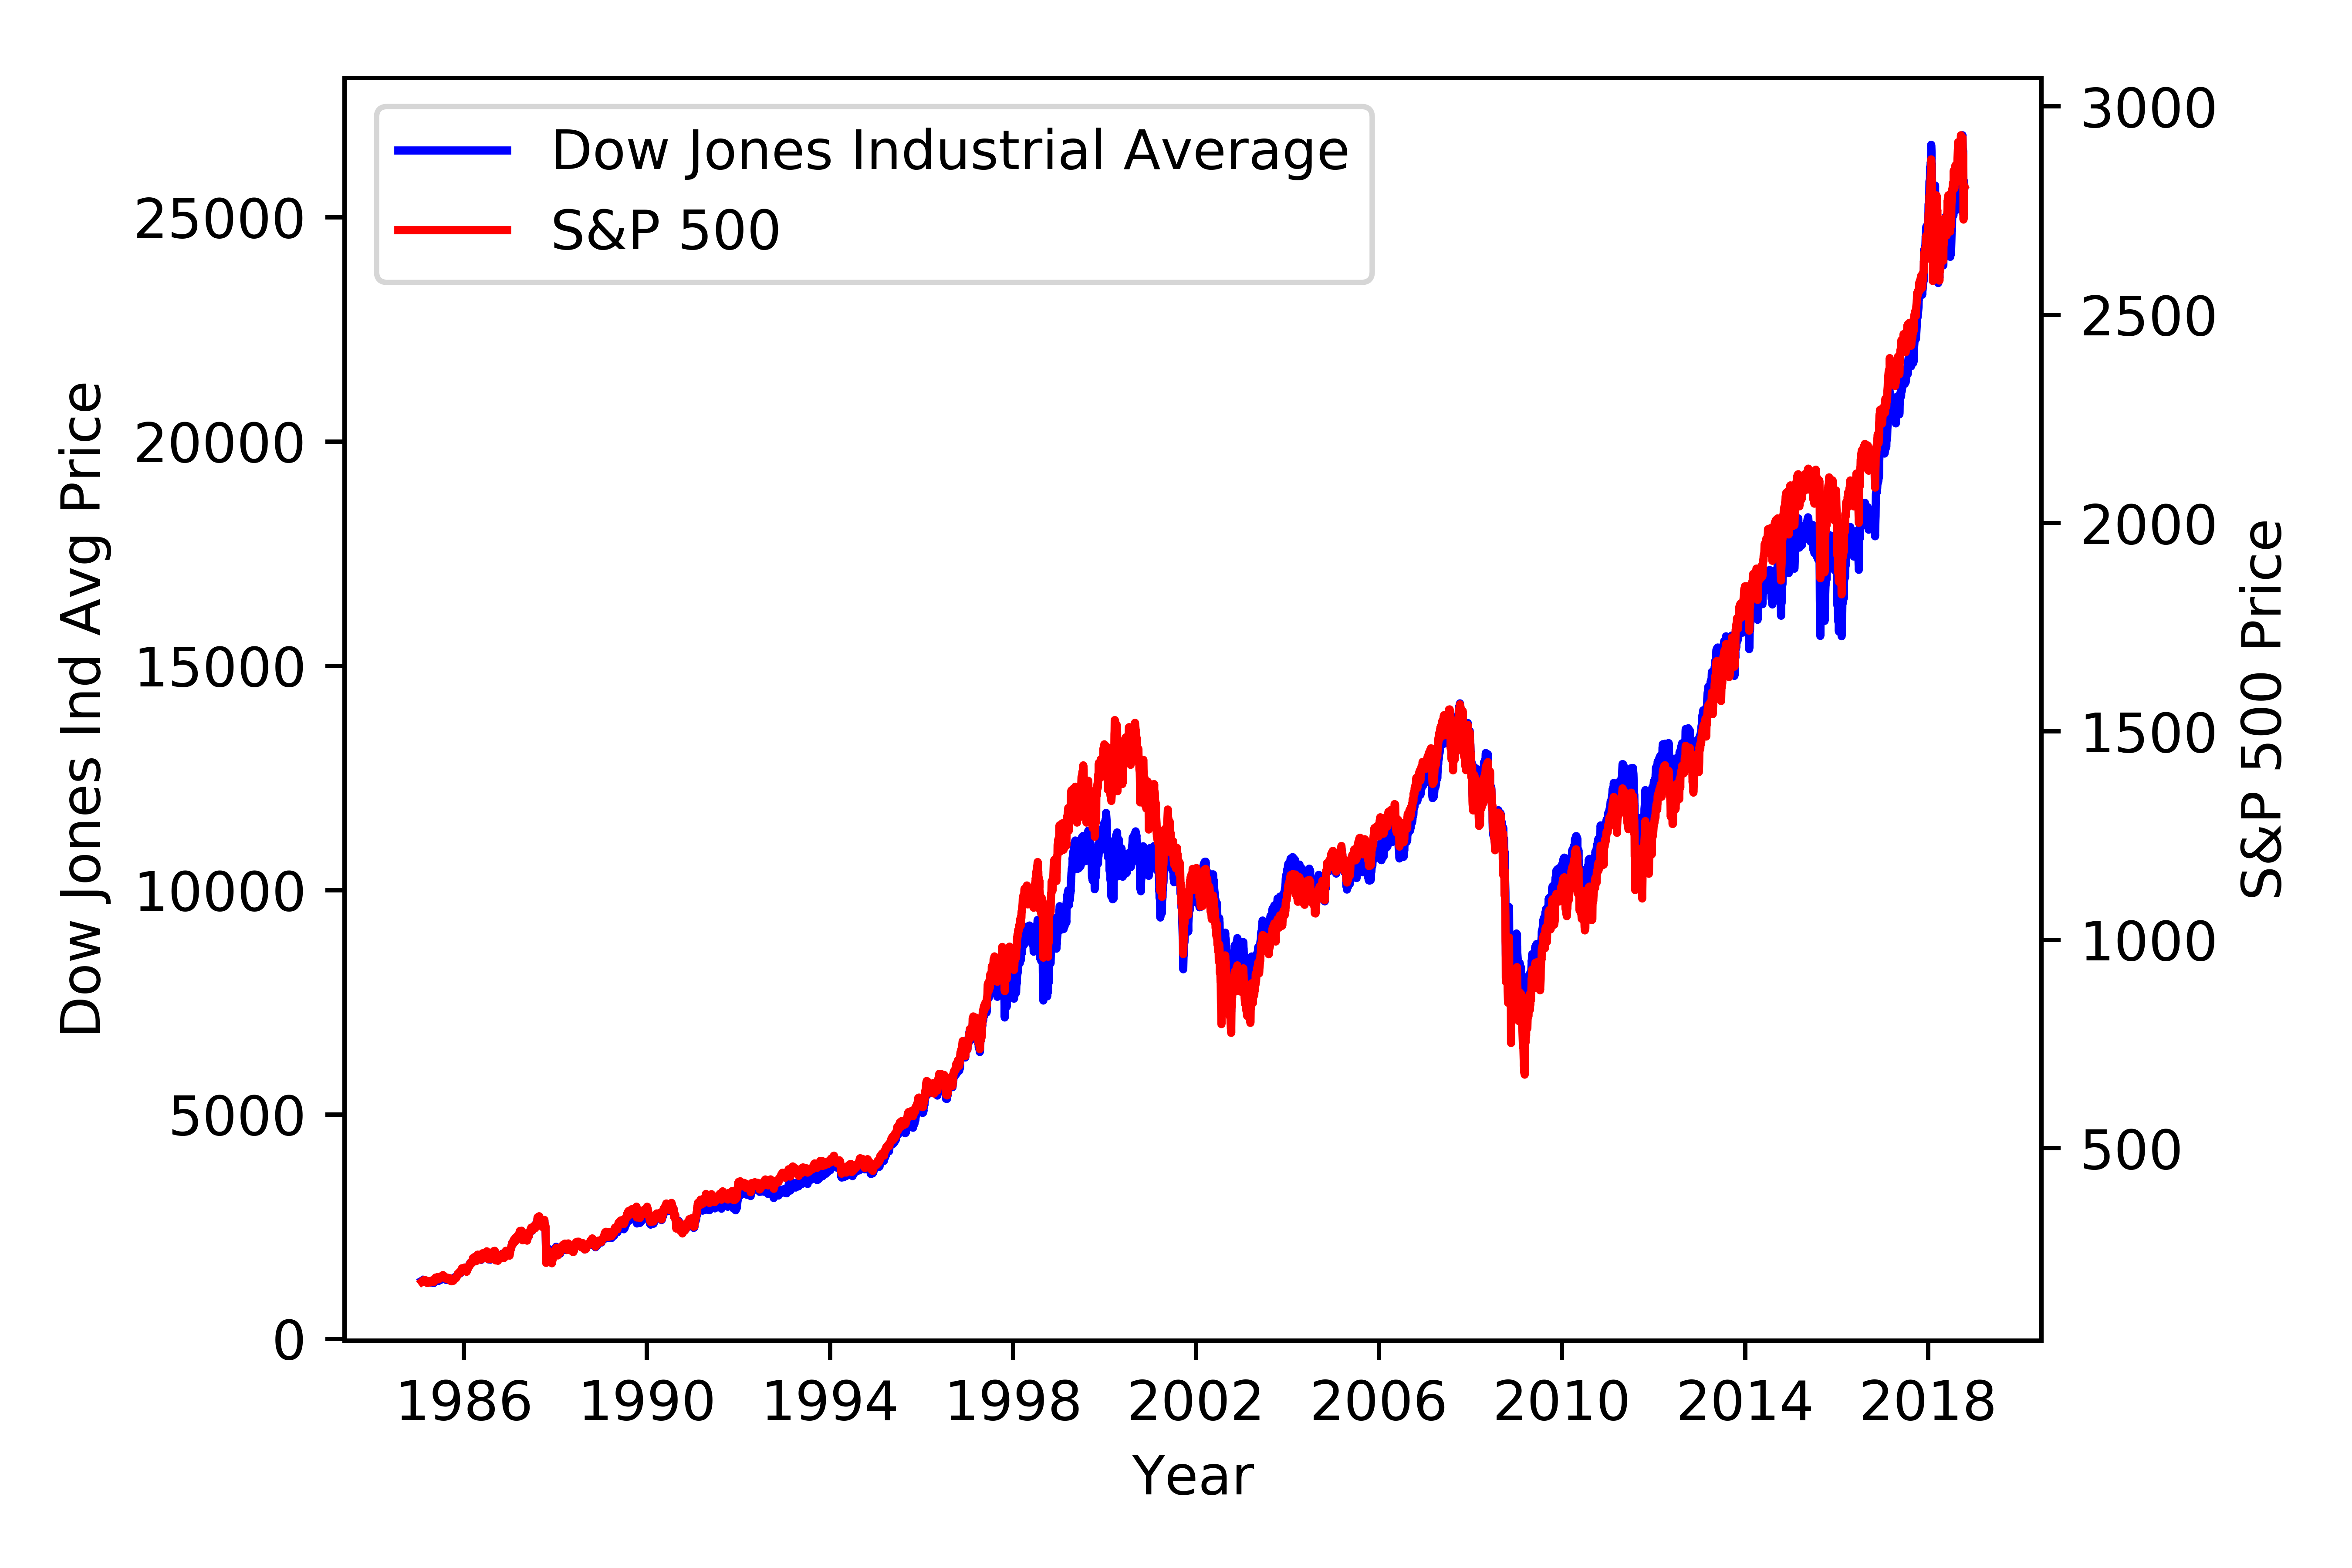
\includegraphics[width=\linewidth]{time_series.png}
	\caption{Time series of Dow Jones and S\%P 500 indexes}
\end{figure}

\subsection{Time series of log returns}


\subsection{Constructing daily log returns}
\begin{figure}[h!]
	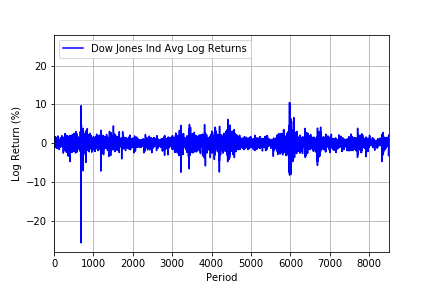
\includegraphics[width=\linewidth]{DJI_logret.png}
	\caption{Time series of Dow Jones Index log return}
\end{figure}
\begin{figure}[h!]
	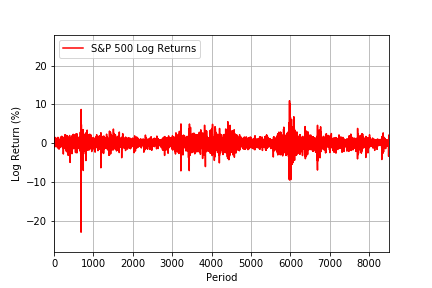
\includegraphics[width=\linewidth]{SP_logret.png}
	\caption{Time series of S\%P 500 log return}
\end{figure}

\subsection{Sample Mean and Sample Variance of log return}
\begin{flushleft}
Sample mean of Dow Jones Index : $ 0.000351774083023244 $ \linebreak 
Sample mean of S\&P 500 Index : $ 0.0003237962025912197 $ \linebreak 
Sample variance of Dow Jones Index : $ 0.00012082440895848629 $ \linebreak 
Sample variance of S\&P 500 Index : $ 0.00012653731363052728 $ \linebreak 
\end{flushleft}




\subsection{Annualized average and volatility of log return}
\begin{flushleft}
Annualized log return of Dow Jones Index : 0.08864706892185749 \linebreak 
Annualized log return of S\&P Index : 0.08159664305298736 \linebreak 
Annualized volatility of Dow Jones Index : 0.17449283955950326 \linebreak 
Annualized volatility of S\&P Index : 0.17857044278069334 \linebreak 
\end{flushleft}

\label{sec:theory}

\subsection{Two-dimensional Electron Gas}
Here, explain the concept of a 2-DEG in GaAs/AlGaAs. What is a 2-DEG and why does it arise?

\subsection{Hall Effect}
Explain the classical Hall effect in your own words. What do I measure at $B=0$? And what happens if $B>0$? Which effect gives rise to the voltage drop in the vertical direction?

\subsection{Quantum Hall Effect}
Explain the IQHE in your own words. What does the density of states look like in a 2-DEG when $B=0$? What are Landau levels and how do they arise? What are edge states? What does the electron transport look like when you change the magnetic field? What do you expect to measure?

\section{Experiment 1-2 pages}
\subsection{Fabrication}
Explain a step-by-step recipe for fabrication here. How long did you etch and why? What is an Ohmic contact?
\subsection{Experimental set-up}
Explain the experimental set-up here. Use a schematic picture (make it yourself in photoshop, paint, ...) to show how the components are connected. Briefly explain how a lock-in amplifier works.

\section{Results and interpretation 2-3 pages}
%Show a graph of the longitudinal resistivity ($\rho_{xx}$) and Hall resistivity ($\rho_{xy}$) versus magnetic field, extracted from the raw data shown in figure \ref{fig:data}. You will have the link to the data in your absalon messages, if not e-mail Guen (guen@nbi.dk). Explain how you calculated these values, and refer to the theory.

\begin{figure}
\centering
% \includegraphics[width=1\textwidth]{raw_data.png}
\caption{\label{fig:data}Raw (unprocessed) data. Replace this figure with the one you've made, that shows the resistivity.}
\end{figure}

\subsection{Classical regime}
Calculate the sheet electron density $n_{s}$ and electron mobility $\mu$ from the data in the low-field regime, and refer to the theory in section \ref{sec:theory}. Explain how you retrieved the values from the data (did you use a linear fit?).
Round values off to 1 or 2 significant digits: 8.1643 ~= 8.2. Also, 5e-6 is easier to read than 0.000005.

!OBS: This part is optional (only if you have time left).
Calculate the uncertainty as follows: \newline $u(f(x, y, z)) = \sqrt{(\frac{\delta f}{\delta{x}} u(x))^{2} + (\frac{\delta f}{\delta{y}} u(y))^{2} + (\frac{\delta f}{\delta{z}} u(z))^{2}}$, where $f$ is the calculated value ($n_{s}$ or $\mu$), $x, y, z$ are the variables taken from the measurement and $u(x)$ is the uncertainty in x (and so on).

\subsection{Quantum regime}
Calculate $n_{s}$ for the high-field regime.
Show a graph of the longitudinal conductivity ($\rho_{xx}$) and Hall conductivity($\rho_{xy}$) \textbf{in units of the resistance quantum} ($\frac{h}{e^{2}}$), depicting the integer filling factors for each plateau.
Show a graph of the plateau number versus its corresponding value of $1/B$. From this you can determine the slope, which you use to calculate the electron density.
Again, calculate the uncertainty for your obtained values.

\section{Discussion 1/2-1 page}
Discuss your results. Compare the two values of $n_{s}$ that you've found in the previous section. Compare your results with literature and comment on the difference. If you didn't know the value of the resistance quantum, would you be able to deduce it from your measurements? If yes/no, why?

\newpage
\section{Some LaTeX tips}
\label{sec:latex}
\subsection{How to Include Figures}

First you have to upload the image file (JPEG, PNG or PDF) from your computer to writeLaTeX using the upload link the project menu. Then use the includegraphics command to include it in your document. Use the figure environment and the caption command to add a number and a caption to your figure. See the code for Figure \ref{fig:frog} in this section for an example.

\begin{figure}
\centering
% \includegraphics[width=0.3\textwidth]{frog.jpg}
\caption{\label{fig:frog}This frog was uploaded to writeLaTeX via the project menu.}
\end{figure}

\subsection{How to Make Tables}

%Use the table and tabular commands for basic tables --- see Table~\ref{tab:widgets}, for example.

\begin{table}
\centering
\begin{tabular}{l|r}
Item & Quantity \\\hline
Widgets & 42 \\
Gadgets & 13
\end{tabular}
\caption{\label{tab:widgets}An example table.}
\end{table}

\subsection{How to Write Mathematics}

\LaTeX{} is great at typesetting mathematics. Let $X_1, X_2, \ldots, X_n$ be a sequence of independent and identically distributed random variables with $\text{E}[X_i] = \mu$ and $\text{Var}[X_i] = \sigma^2 < \infty$, and let

\begin{equation}
S_n = \frac{X_1 + X_2 + \cdots + X_n}{n}
      = \frac{1}{n}\sum_{i}^{n} X_i
\label{eq:sn}
\end{equation}

denote their mean. Then as $n$ approaches infinity, the random variables $\sqrt{n}(S_n - \mu)$ converge in distribution to a normal $\mathcal{N}(0, \sigma^2)$.

%The equation \ref{eq:sn} is very nice.

\subsection{How to Make Sections and Subsections}

Use section and subsection commands to organize your document. \LaTeX{} handles all the formatting and numbering automatically. Use ref and label commands for cross-references.

\subsection{How to Make Lists}

You can make lists with automatic numbering \dots

\begin{enumerate}
\item Like this,
\item and like this.
\end{enumerate}
\dots or bullet points \dots
\begin{itemize}
\item Like this,
\item and like this.
\end{itemize}
\dots or with words and descriptions \dots
\begin{description}
\item[Word] Definition
\item[Concept] Explanation
\item[Idea] Text
\end{description}

We hope you find write\LaTeX\ useful, and please let us know if you have any feedback using the help menu above.

\begin{thebibliography}{9}
\bibitem{nano3}
  K. Grove-Rasmussen og Jesper Nygård,
  \emph{Kvantefænomener i Nanosystemer}.
  Niels Bohr Institute \& Nano-Science Center, Københavns Universitet

\end{thebibliography}
\end{document}